%\documentclass[acmsmall,review,nonacm]{acmart}\settopmatter{printfolios=true,printccs=false,printacmref=false}
\documentclass[acmsmall,nonacm]{acmart}
%%
%% \BibTeX command to typeset BibTeX logo in the docs
\AtBeginDocument{%
	\providecommand\BibTeX{{%
			\normalfont B\kern-0.5em{\scshape i\kern-0.25em b}\kern-0.8em\TeX}}}

%% Rights management information.  This information is sent to you
%% when you complete the rights form.  These commands have SAMPLE
%% values in them; it is your responsibility as an author to replace
%% the commands and values with those provided to you when you
%% complete the rights form.
\setcopyright{acmcopyright}
\copyrightyear{2018}
\acmYear{2018}
\acmDOI{10.1145/1122445.1122456}

% for code
\usepackage{listings}
\usepackage{lipsum}
\usepackage{xcolor}
\usepackage{minted}
\RecustomVerbatimEnvironment{Verbatim}{BVerbatim}{}

% tables
\usepackage{multirow}


%% These commands are for a PROCEEDINGS abstract or paper.
\acmConference[Woodstock '18]{Woodstock '18: ACM Symposium on Neural
	Gaze Detection}{June 03--05, 2018}{Woodstock, NY}
\acmBooktitle{Woodstock '18: ACM Symposium on Neural Gaze Detection,
	June 03--05, 2018, Woodstock, NY}
\acmPrice{15.00}
\acmISBN{978-1-4503-XXXX-X/18/06}


%%
%% Submission ID.
%% Use this when submitting an article to a sponsored event. You'll
%% receive a unique submission ID from the organizers
%% of the event, and this ID should be used as the parameter to this command.
%%\acmSubmissionID{123-A56-BU3}

%%
%% The majority of ACM publications use numbered citations and
%% references.  The command \citestyle{authoryear} switches to the
%% "author year" style.
%%
%% If you are preparing content for an event
%% sponsored by ACM SIGGRAPH, you must use the "author year" style of
%% citations and references.
%% Uncommenting
%% the next command will enable that style.
%%\citestyle{acmauthoryear}

%%
%% end of the preamble, start of the body of the document source.
\begin{document}
	
	%%
	%% The "title" command has an optional parameter,
	%% allowing the author to define a "short title" to be used in page headers.
	\title{Fine-grained Reductions Around CFL reachability}
	
	%%
	%% The "author" command and its associated commands are used to define
	%% the authors and their affiliations.
	%% Of note is the shared affiliation of the first two authors, and the
	%% "authornote" and "authornotemark" commands
	%% used to denote shared contribution to the research.
	\author{Aleksandra Istomina}
	\thanks{Aleksandra Istomina: graduate student, email: aleksandra2999@mail.ru, ACM student member number: 4678238}
	\email{aleksandra2999@mail.ru}
	\affiliation{%
		\institution{Saint Petersburg State University}
		\city{Saint Petersburg}
		\country{Russia}
	}
	\affiliation{%
		\institution{JetBrains Research}
		\city{Saint Petersburg}
		\country{Russia}
	}
	
	\author{Research advisor: Semyon Grigorev}
	\affiliation{%
		\institution{Saint Petersburg State University}
		\city{Saint Petersburg}
		\country{Russia}
	}
	\affiliation{%
		\institution{JetBrains Research}
		\city{Saint Petersburg}
		\country{Russia}
	}
	
	\newcommand\todo[1]{{\color{violet}#1}}
	\newcommand\db[1]{{\color{red}#1}}
	\newcommand\question[1]{{\color{cyan}#1}}
	
	%%
	%% By default, the full list of authors will be used in the page
	%% headers. Often, this list is too long, and will overlap
	%% other information printed in the page headers. This command allows
	%% the author to define a more concise list
	%% of authors' names for this purpose.
	% \renewcommand{\shortauthors}{Trovato and Tobin, et al.}
	
	%%
	%% The abstract is a short summary of the work to be presented in the
	%% article.
	
	
	%%
	%% The code below is generated by the tool at http://dl.acm.org/ccs.cfm.
	%% Please copy and paste the code instead of the example below.
	%%
	\begin{CCSXML}
		<ccs2012>
		<concept>
		<concept_id>10003752.10003766.10003771</concept_id>
		<concept_desc>Theory of computation~Grammars and context-free languages</concept_desc>
		<concept_significance>500</concept_significance>
		</concept>
		<concept>
		<concept_id>10003752.10010124.10010138.10010143</concept_id>
		<concept_desc>Theory of computation~Program analysis</concept_desc>
		<concept_significance>500</concept_significance>
		</concept>
		%<concept>
		%<concept_id>10002950.10003624.10003633.10003640</concept_id>
		%<concept_desc>Mathematics of computing~Paths and connectivity problems</concept_desc>
		%<concept_significance>300</concept_significance>
		%</concept>
		<concept>
		<concept_id>10003752.10003777.10003779</concept_id>
		<concept_desc>Theory of computation~Problems, reductions and completeness</concept_desc>
		<concept_significance>500</concept_significance>
		</concept>
		</ccs2012>
	\end{CCSXML}
	
	\ccsdesc[500]{Theory of computation~Grammars and context-free languages}
	\ccsdesc[500]{Theory of computation~Program analysis}
	%\ccsdesc[300]{Mathematics of computing~Paths and connectivity problems}
	\ccsdesc[500]{Theory of computation~Problems, reductions and completeness}
	
	%%
	%% Keywords. The author(s) should pick words that accurately describe
	%% the work being presented. Separate the keywords with commas.
	% \keywords{datasets, neural networks, gaze detection, text tagging}
	
	
	%%
	%% This command processes the author and affiliation and title
	%% information and builds the first part of the formatted document.
	\maketitle
	
	\section{Introduction}
	
	Context-free language (CFL) reachability is a framework for graph analysis which was introduced by Thomas Reps~\cite{REPS1998701} and allows one to specify path constraints in terms of context-free languages. CFL reachability finds application in such fields of research as static code analysis (e.g. type-based flow analysis~\cite{10.1145/373243.360208} or points-to analysis~\cite{10.1145/1103845.1094817, 10.1145/1133255.1134027}), graph databases~\cite{10.1145/298514.298576}, bioinformatics~\cite{SubgraphQueriesbyContextfreeGrammars}.
	
	There are several cubic~\cite{10.1145/298514.298576, 10.1145/199448.199462} and slightly subcubic~\cite{10.1145/1328438.1328460} (with time $\mathcal{O}(n^{3} / \log n)$) algorithms for CFL reachability. The big open question is whether a truly subcubic (with time $\tilde{\mathcal{O}}(n^{3 - \epsilon}) = \mathcal{O}(n^{3 - \epsilon} \cdot polylog(n))$) algorithm exists. 
	
	One of the ways to answer that question is to make a fine-grained reduction from other problem that is known or strongly believed to have some lower bound to CFL reachability problem. In that case CFL reachability problem will have non-trivial conditional lower bound as faster algorithm for it will lead to faster algorithm for other problem. Currently there are several fine-grained complexity results in this area, but they are scattered and have no structure.
	
	In this paper we give an overview on these existing results: what is already achieved and what questions are still to be answered.
	
	\section{Preliminaries}
	
	\emph{Context-free grammar} (CFG) is a four $G=(N, \Sigma, P, S)$, where $N$ is a set of nonterminals, $\Sigma$ is a set of terminals, $P$ is a set of productions of the followings form: $A \to \alpha$, $\alpha \in (N \cup \Sigma)^*$ ans $S$ is a starting nonterminal. Denote a context-free language of words derived from the starting symbol as $L(G)$.
	
	\emph{CFG recognition} problem is to decide whether $w \in L(G)$ given a CFG $G$ and a string $w \in \Sigma^*$. This problem is closely related to \emph{CFG parsing problem} where we want a possible derivation sequence, if $w \in L(G)$. It is known~\cite{10.5555/646233.682379} that CFG recognition is as hard as CFG parsing up to logarithmic factors.
	
	Let $D = (V, E, L)$ be a directed graph which edges are labelled with symbols from $L \subseteq \Sigma$. We call a path from vertex $v$ to vertex $u$ an $S$-path if concatenation of labels on that path is a word from $L(G)$.  \emph{Context-free language (CFL) reachability} problem~\cite{REPS1998701} is to determine if there exists an $S$-path between a given sets of vertices $A, B$. In \emph{single source/single target (s-t)} CFL reachability $A = \{s\}, B = \{t\}, s, t \in V(D)$. In \emph{all-pairs} CFL reachability $A = B = V(D)$.
	
	\emph{Dyck-$k$} reachability problem is a CFL reachability problem where $G$ defines a Dyck language on $k$ types of parentheses. The corresponding grammar is $G=(N, \Sigma, P, S)$, where $N = \{S\}, \Sigma = \{(_i, )_i\}, \forall i = 1, \ldots, k$, productions rules are $S \rightarrow \epsilon | SS | (_1 S )_1 | \ldots | (_k S )_k$, where $\epsilon$ is the empty string. 
	
	For problems $P, Q$ and time bounds $t_P, t_Q$, a \emph{fine-grained reduction}~\cite{bringmann2019fine} from $(P, t_P)$ to $(Q, t_Q)$ is an algorithm that, given an instance $I$ of $P$, computes an instance $J$ of $Q$ such that: 
	
	\begin{itemize}
		\item $I$ is a YES-instance of $P$ if and only if $J$ is a YES-instance of $Q$,
		\item for any $\epsilon > 0$ there is a $\delta > 0$ such that $t_Q(|J|)^{1 - \epsilon} = \mathcal{O}(t_P (|I|)^{1 - \delta})$, 
		\item the running time of the reduction is $\mathcal{O}(t_P (|I|)^{1 - \gamma})$ for some $\gamma > 0$.
	\end{itemize}
	
	
	\section{Main Results}
	
	This section is organised as follows. Firstly, we define fine-grained complexity problems which we use later. Secondly we present a map of existing fine-grained reductions and make an overview of some selected ones. After that we discuss some open problems. 
	
	\begin{figure}[!htp]
		
		\begin{center}  
			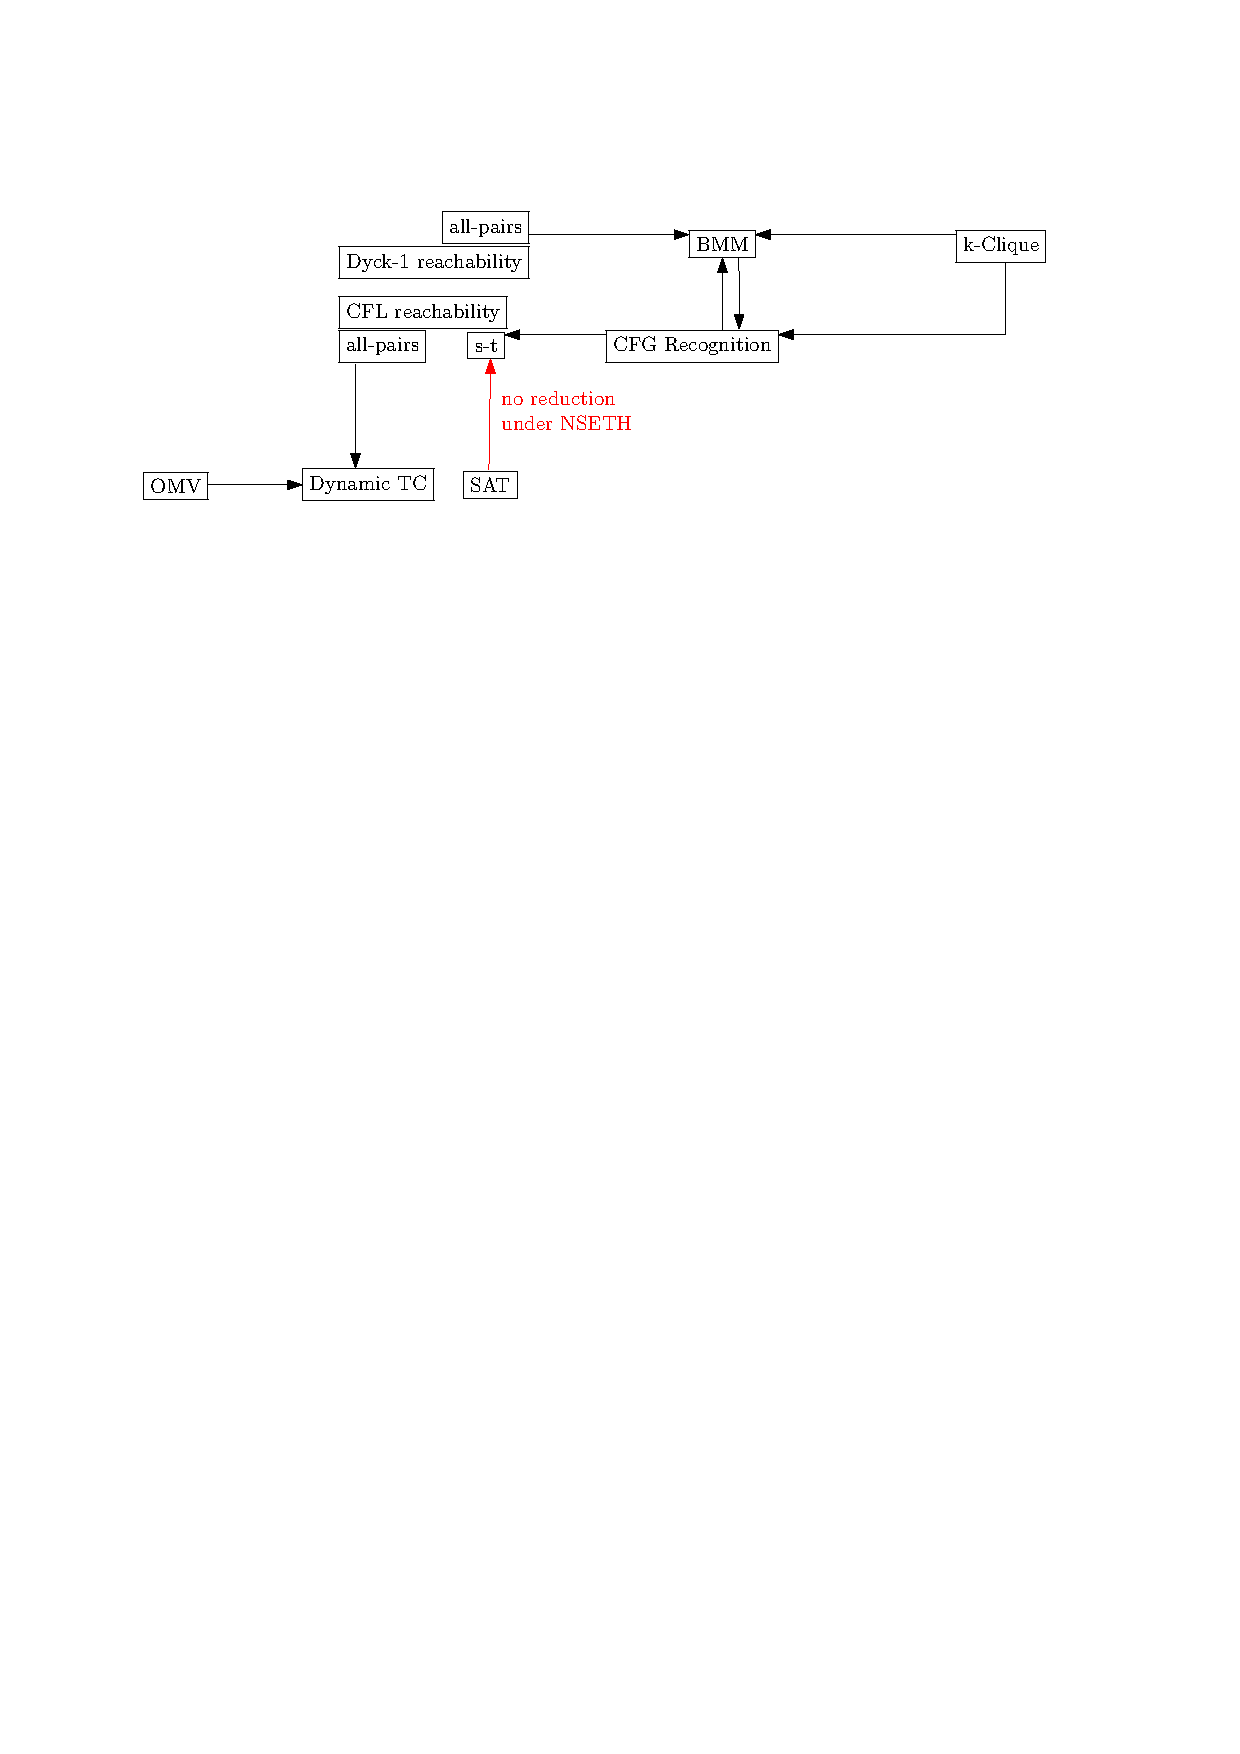
\includegraphics[scale = 0.6]{map_popl.pdf}
		\end{center}
		
		\caption{Existing reductions concerning CFL reachability and CFG recognition. Black arrow $a \rightarrow b$ represents existing reduction from $a$ to $b$. Red arrow analogously represents non-existence of the reduction. }
		\label{fig:map}
		
	\end{figure}
	
	\subsection{Existing problems and hypotheses}
	
	%There are several problems that are connected with CFL recognition and reachability. 
	
	\emph{Boolean satisfiability problem (SAT, $k$-SAT)} is to determine if there exists an interpretation of variables that satisfies a given Boolean formula on $n$ variables written in $k$-CNF, $k > 3$. The hypothesis about SAT, that we are interested about, is NSETH~\cite{10.1145/2840728.2840746} which proposes that there is no $\epsilon > 0$ such that $k$-SAT can be solved co-nondeterministically in time $2^{(1 - \epsilon) n}$ for any $k$.
	
	In \emph{Boolean Matrix Multiplication (BMM)} problem it is needed to calculate matrix product of the two given $n \times n$ matrices over (AND, OR). BMM hypothesis states that there is no $\mathcal{O}(n^{3 - \epsilon})$ combinatorial algorithm for that. 
	
	\emph{Orthogonal Vectors (OV)} problem decides whether two sets $X, Y$ of $n$ boolean $d$-dimensional vectors contain a pair $x \in X, y \in Y$ which dot product equals zero. Hypothesis states that OV problem cannot be solved in $\mathcal{O}(n^{2 - \epsilon} \cdot poly(d))$ time. 
	
	Given an undirected graph $U$ on $n$ vertices the \emph{$k$-Clique} problem~\cite{abboud2018if} seeks the clique on $k$ vertices in $U$.  If $0 \leq F \leq \omega$ and $0 \leq C \leq 3$ are the smallest numbers such that $3k$-Clique can be solved combinatorially in $\mathcal{O}(n^{Ck})$ time and in $\mathcal{O}(n^{Fk})$ time by any algorithm, for any constant $k \geq 1$, a conjecture is that $C = 3$ and $F = \omega$.
	
	In the \emph{Online boolean Matrix-Vector multiplication (OMV)} problem~\cite{10.1145/2746539.2746609} we are given an $n \times n$ boolean matrix $M$, we receive $n$ boolean vectors $v_1, \ldots, v_n$ one at a time, and are required to output $Mv_i$ (over the boolean semiring) before seeing the vector $v_{i+1}$, for all $i$. It is conjectured that there is no algorithm with total time $\mathcal{O}(n^{3-\epsilon})$, even with polynomial time to preprocess $M$.
	
	The incremental \emph{Dynamic Transitive Closure (DTC)}~\cite{Hanauer2020FasterFD} problem asks to maintain reachability information in a directed graph $D = (V, E)$ between arbitrary pairs of vertices under insertions of edges. Conditional lower bound on DTC follows from OMV hypothesis and reduction from it~\cite{10.1145/2746539.2746609}: there is no algorithm with total update time $\mathcal{O}((mn)^{1 - \epsilon})$ ($n = |V|, m = |E|$) even with $poly(n)$ time preprocessing of the input graph and $m^{\delta - \epsilon}$ query time per query for any $\delta \in (0, 1/2]$ such that $m = \Theta(n^{1/(1-\delta)})$ under OMV hypothesis.
	
	\subsection{Existing reductions}
	
	First of all we need to mention the interconvertibility of CFL reachability problems and a class of set-constraint problems~\cite{10.1145/258994.259006} as this result allows us to reformulate our problem if we wish so.
	
	One of the interesting reductions was a reduction from  all-pairs Dyck-1 reachability problem to BMM problem. It was firstly proved by Bradford~\cite{bradford2017efficient} via algebraic matrix encoding and then combinatorially by Mathiasen and Pavlogiannis~\cite{10.1145/3434315} by combining Dyck-1 path from bell-shaped paths. For this and the following reductions see Fig.~\ref{fig:map}.
	
	In the recent paper of Shemetova et al.~\cite{shemetova2021algorithm} the reduction from all-pairs CFL reachability to incremental DTC have been proven. Still this reduction cannot give truly subcubic algorithm for CFL reachability without refuting OMV conjecture~\cite{8948597, 10.1145/2746539.2746609}.
	
	The following results are the most interesting ones concerning the existence of  the truly subcubic algorithm for CFL reachability.
	
	The CFL reachability problem has been shown to be 2NPDA-complete~\cite{10.5555/788019.788876}. It means that subcubic algorithm for CFL reachability would lead to subcubic algorithms for the whole 2NPDA class and cubic upper bound has not been improved since the discovery of the class in 1968.
	
	Non-existence of the truly subcubic combinatorial algorithm for \emph{s-t} CFL reachability under BMM hypothesis was proved by combining two reductions: the combinatorial reduction from CFG recognition to \emph{s-t} CFL reachability~\cite{10.1145/3158118} and combinatorial reduction from BMM to CFG Recognition~\cite{10.1145/505241.505242}.
	
	Recently it was discovered by Chistikov et al.~\cite{chistikov2021subcubic} that there exist subcubic certificates for \emph{s-t} CFL reachability (for existence and non-existence of the valid paths). From this fact it follows that there are no reductions under NSETH from SAT problem to CFL reachability problem that give lower bound stronger than $\mathcal{O}(n^{\omega})$.
	
	\subsection{Open problems}
	
	The equivalence under subcubic reduction of \emph{s-t} and 
	all-pairs CFL reachability is not yet discovered. However the analogous result for triangle detection in a graph is true~\cite{10.1145/3186893} and, perhaps, similar techniques are applicable in our area. 
	
	Currently there is no non-trivial lower bound on Dyck-1 reachability problem. 
	Yet we know that there exists a reduction from OV problem to Andersen pointer analysis~\cite{10.1145/3434315} where as a part of reduction appears slightly modified Dyck-1 reachability with an additional if-condition for edge existence in a graph. If similar reduction to pure Dyck-1 reachability problem exists it would give conditional quadratic lower bound. 
	
	Finding a fine-grained reduction from all-pairs shortest paths (APSP) problem or OMV problem to CFL reachability problem would give a conditional lower bound on it's complexity. We highlight APSP problem and it's subcubic equivalent analogues~\cite{10.1145/3186893} as APSP is connected to problems on paths, and OMV problem as it is connected to dynamic problems as is CFL reachability problem. 
	
	\section{Conclusion and Future work}
	
	In this paper we have collected existing results in fine-grained complexity concerning CFL reachability and CFG recognition problems. We have presented existing reductions and some open problems with intuition for possible ways of their solution. 
	
	To summarize, CFL reachability is a popular problem strongly connected with many areas. It has several cubic algorithms and no truly subcubic combinatorial one under BMM hypothesis. It has been proved that we cannot get cubic lower bound on CFL reachability using reduction from SAT under NSETH. Still other reductions may be possible, e.g. from APSP or OMV problems. 
	
	Getting cubic conditional lower bound through some hypothesis is a possible way of future work as is closing other open problems. In our overview, we have reached the DTC problem, which lies in a field of dynamic problems, alongside with many other problems and reductions of our interest. In the future, we plan to investigate these directions. 
	
	\section{Acknowledgments}
	
	The research was supported by the Russian Science Foundation, grant \textnumero 18-11-00100.
	
	\bibliographystyle{ACM-Reference-Format}
	\bibliography{map}
	
	%%
	%% If your work has an appendix, this is the place to put it.
	%\appendix
	
\end{document}
\endinput